\chapter{考虑机间避碰与通信保持的编队控制方法}

\section{控制目标描述}
考虑在 $n$ 维空间中运行的 $N$ 架无人机，每架无人机的动态特性可由单积分器模型(\ref{位置导数等于速度})描述。为了在协同编队过程中实现机间避碰并保持网络通信连通性，考虑连通的通信拓扑$\mathcal{G} = (\mathcal{V}, \mathcal{E})$，相邻无人机之间的距离 $\|\mathbf{p}_i - \mathbf{p}_j\|$ 必须严格满足以下约束条件：
\begin{equation}
	\rho_{e_1} \le \|\mathbf{p}_i - \mathbf{p}_j\| \le \rho_{e_2}, \quad 0 < \rho_{e_1} < \rho_{e_2}.
	\label{距离约束条件}
\end{equation}
在此约束中， $\rho_{e_1}$ 代表避免无人机发生碰撞的安全距离下界，而 $\rho_{e_2}$ 则代表保证机间可靠通信的距离上界。

本章的核心控制目标是：针对具有期望无穷小刚性框架 $\mathcal{F}^* = (\mathcal{G}, \mathbf{p}^*)$ 的多智能体系统，在仅依赖局部测距和部分节点非全维绝对位置量测的情况下，设计分布式观测器与控制器，使得系统能够局部渐近收敛至期望编队位置 $\mathbf{p}^*$，并在整个收敛过程中始终满足公式中所述的机间避碰与通信保持约束。

\section{控制协议设计}

\subsection{分布式观测器设计}
首先考虑无人机$i$在期望点$\mathbf{p}_i^*$附近的位置估计。为了方便推导反馈增益矩阵，将无人机编队系统在期望位置${\mathbf{p}}^*$处的刚性矩阵$\mathcal{R}_{\mathbf{p}^*}$按照无人机索引分解为：
\begin{equation}
	\mathcal{R}_{\mathbf{p}^*} = 
	[\bar{C}_1,\cdots,\bar{C}_i,\cdots,\bar{C}_N],
	\quad
	\bar{C}_i \in \mathbb{R}^{M \times n}.
\end{equation}
接着矩阵$\bar{C}_i$和位置输出矩阵$\tilde{C}_i$可以联合组成无人机$i$的线性化输出矩阵：
\begin{equation}
	C_i = 
	\begin{bmatrix}
		\bar{C}_i \\
		\tilde{C}_i
	\end{bmatrix}.
	\label{非全维位置输出矩阵}
\end{equation}
由期望位置组成的刚性矩阵$\mathcal{R}_{\mathbf{p}^*}$是已知且固定的，这使得该方法仅具备局部收敛性。

由于部分无人机无法直接获取全局坐标系下的全维位置，系统需要通过观测器来估计自身位置。令 $\hat{\mathbf{p}}_i$ 表示第 $i$ 架无人机在全局坐标系中的位置估计值。基于式(\ref{非全维位置输出矩阵})非全维位置输出矩阵${C}_i$，提出如下分布式观测器设计：
\begin{equation}
	\dot{\hat{\mathbf{p}}}_i = \mathbf{v}_i + k_o {C}_i^\top \left[ (\mathbf{z}_i - \mathbf{z}_i^*) - \sum_{j \in \{i, \mathcal{N}_i\}} {C}_j (\hat{\mathbf{p}}_j - \hat{\mathbf{p}}_i) \right],
	\label{分布式观测器}
\end{equation}
其中， $k_o$ 为观测器反馈增益， $\mathbf{z}_i^*$ 为系统在期望位置 $\mathbf{p}^*$处的输出量测，$\mathbf{z}_i^*=[{\bar{\mathbf{z}}_i}^*;{\tilde{\mathbf{z}}_i}^*]$，${\bar{\mathbf{z}}_i}^*=\frac{1}{2}[\cdots;|h_{im}|\beta_{ij};\cdots]$以及${\tilde{\mathbf{z}}_i}^*=\tilde{C}_i \mathbf{p}_i^*$，$\mathcal{N}_i$ 为通信拓扑中节点 $i$ 的邻居集合。该观测器通过融合传感器量测输出与邻居节点的估计信息，实现对全局位置的渐近观测。

\subsection{分布式控制器设计}
为了引导无人机$i$收敛至期望位置$\mathbf{p}^*$，基础的反馈控制律可设计为位置估计误差的线性反馈：
\begin{equation}
	\tilde{\mathbf{v}}_i^* = 
	-k_c (\hat{\mathbf{p}}_i - \mathbf{p}^*_i),
	\label{反馈控制律}
\end{equation}
式中控制增益$k_c$需满足的条件将会在后续控制器设计内容中给出。

然而，在缺乏全局坐标系的集群作业中，保持编队的几何刚性是实现稳定编队的前提 \cite{7074770}。基于人工势函数的梯度下降法是解决此类问题的经典范式，通过最小化个体与其邻居间的配置误差来驱动全局状态收敛\cite{10.1016/j.automatica.2011.08.019}。梯度控制律通常由具体设计的势函数表征：
\begin{equation}
	\nu_i(\mathbf{p}_i,\cdots,\mathbf{p}_j,\cdots)=
	\sum_{j \in  \mathcal{N}_i} \gamma_{ij} (\beta_{ij}),
\end{equation}
式中$\gamma_{ij}(\cdot):\mathbb{R} \to \bar{\mathbb{R}}_+$是正定且在平衡点$\beta_{ij}^*=\|\mathbf{p}_i^* - \mathbf{p}_j^*\|^2$ 的邻域内具有解析形式。为了简洁叙述，后续将使用符号$\gamma_{ij}=\gamma_{ij} (\beta_{ij})$以及$\nu_i=\nu_i(\mathbf{p}_i,\cdots,\mathbf{p}_j,\cdots)$。此时，无人机$i$梯度控制律的解析形式可以写为：
\begin{align}
	\bar{\mathbf{v}}_i^* = 
	-\frac{1}{2} \nabla_{\mathbf{p}_i} \nu_i = 
	- \underbrace{
		\sum_{j \in  \mathcal{N}_i} \frac{\partial \gamma_{ij}}{\partial \beta_{ij}}
		}
		_{\text{距离相关项}}
	\underbrace{(\mathbf{p}_i - \mathbf{p}_j)}_{\text{相对位移项}},
	\label{梯度控制律}
\end{align}
该式中距离相关项驱动无人机编队的距离收敛，而相对位移项提供方向引导。对于一阶积分器组成的多智能体系统，现有研究已证实控制律(\ref{梯度控制律})能够驱动系统局部收敛至编队集合且保持一阶刚性\cite{7074770,Kwang2014Distance,https://doi.org/10.1002/rnc.3477}：
\begin{equation}
	E = \{ \mathbf{p} \in \mathbb{R}^{Nn} : 
	\|\mathbf{p}_i - \mathbf{p}_j\| = 
	\|\mathbf{p}_i^* - \mathbf{p}_j^*\|,
	\quad
	\forall i,j \in \mathcal{I}_{N}
	\}
\end{equation}

本文的核心目标之一是确保无人机系统(\ref{一阶动力学})在收敛至期望编队位置的同时保持无穷小刚性，因此可将控制律(\ref{反馈控制律})$\tilde{\mathbf{v}}_i^*$和(\ref{梯度控制律})$\bar{\mathbf{v}}_i^*$进行结合。另外注意到本文的传感器条件中，无人机$i$无法获取全维位置下的绝对位置，因而机间相对位移项$\mathbf{p}_i - \mathbf{p}_j$无法直接进行获取，将其替换为估计值$\hat{\mathbf{p}}_i - \hat{\mathbf{p}}_j$，便可以得到一种耦合的控制律：
\begin{equation}
	\mathbf{v}_i^* = 
	-\sum_{j \in  \mathcal{N}_i} \frac{\partial \gamma_{ij}}{\partial \beta_{ij}} (\hat{\mathbf{p}}_i - \hat{\mathbf{p}}_j) 
	-k_c (\hat{\mathbf{p}}_i - \mathbf{p}^*_i).
	\label{耦合控制律}
\end{equation}

接下来讨论函数$\gamma_{ij}$的具体数学形式。通常情况下，函数$\gamma_{ij}$具有二次项形式：
\begin{equation}
	\bar{\gamma}_{ij} = k_\gamma (\beta_{ij}-\beta_{ij}^*)^2,
	\quad
	k_\gamma > 0.
\end{equation}
其中 $k_\gamma > 0$ 为函数$\gamma_{ij}$的常数参数。该式仅保证距离的收敛性特性，但未考虑收敛过程中的距离约束问题。为了保证无人机编队在收敛过程中同时满足距离约束(\ref{距离约束条件})，可以设计函数$ \tilde{\gamma}_{ij} $：
\begin{equation}
	\tilde{\gamma}_{ij} = 
	k_\gamma[
		(\beta_{ij}-\beta_{ij}^*)^2 - 
		\ln (\beta_{ij}-\rho_{e_1}^2) - 
		\ln (\rho_{e_2}^2-\beta_{ij})
	].
\end{equation}
进一步，为使$\beta_{ij}=\beta_{ij}^*$成为函数$\gamma_{ij}$的平衡点，在接近边界条件时势能趋于无穷大，同时确保势函数$\nu_i$的正定性，即$\gamma_{ij} \ge 0$并且$\frac{\partial \gamma_{ij}}{\partial \beta_{ij}}(\beta_{ij}^*)=0$。函数$\tilde{\gamma}_{ij}$可进一步修正为：
\begin{equation}
	\gamma_{ij} = k_\gamma \left[ (\beta_{ij} - \beta_{ij}^*)^2 + \ln \frac{(\rho_{e_2}^2 - \beta_{ij}^*)(\beta_{ij}^* - \rho_{e_1}^2)}{(\rho_{e_2}^2 - \beta_{ij})(\beta_{ij} - \rho_{e_1}^2)}  + \frac{(\rho_{e_2}^2 - 2\beta_{ij}^* + \rho_{e_1}^2)(\beta_{ij} - \beta_{ij}^*)}{(\rho_{e_2}^2 - \beta_{ij}^*)(\beta_{ij}^* - \rho_{e_1}^2)}
	\right].
	\label{gamma函数}
\end{equation}
接着将公式(\ref{gamma函数})带入公式(\ref{耦合控制律})，可以推导出分布式控制律：
\begin{equation}
	\mathbf{v}_i^* = 
	- \sum_{j \in \mathcal{N}_i} \gamma_{ij}' (\hat{\mathbf{p}}_i - \hat{\mathbf{p}}_j) 
	- k_c (\hat{\mathbf{p}}_i - {\mathbf{p}}_i^*),
	\label{分布式控制律}
\end{equation}
其中
\begin{equation}
	\gamma_{ij}' = 
	k_\gamma \left[ 2(\beta_{ij} - \beta_{ij}^*) + 
	\frac{\rho_{e_1}^2+\rho_{e_2}^2-2\beta_{ij}}{(\rho_{e_2}^2-\beta_{ij}^*)(\beta_{ij}^* - \rho_{e_1}^2)}  + 
	\frac{\rho_{e_2}^2-2\beta_{ij}^*+\rho_{e_1}^2}{(\rho_{e_2}^2-\beta_{ij}^*)(\beta_{ij}^*-\rho_{e_1}^2)}
	\right].
\end{equation}
在该分布式控制律(\ref{分布式控制律})中，第一项为基于势函数梯度的相对位移控制项，主要作用是驱使无人机保持预设距离从而实现避碰和防失联；第二项则是位置反馈控制项，利用控制增益$k_c$引导编队系统整体收敛至期望参考位置 $\mathbf{p}_i^*$。

为了直观理解上述函数的特性，图\ref{不同伽马函数的对比曲线}绘制了上述函数的对比曲线，其中$\rho_{e_1}=0.5m$，$\rho_{e_2}=2m$以及$\beta_{ij}^*=2 m^2$。从图中可以看出函数$\bar{\gamma}_{ij}$和$\gamma_{ij}$均大于等于0，并且在$\beta_{ij}=\beta_{ij}^*$处有极小值0，而函数$\tilde{\gamma}_{ij}$并非正定且极值不在$\beta_{ij}=\beta_{ij}^*$处。此外，函数$\gamma_{ij}$与$\tilde{\gamma}_{ij}$均具备边界性质：
\begin{equation}
	\lim_{\beta_{ij} \to \{(\rho_{e_1}^2)_+, (\rho_{e_2}^2)_-\} } \left| \frac{\partial \gamma_{ij}}{\partial \beta_{ij}} \right| \to \infty,
	\quad
	\lim_{\beta_{ij} \to \{(\rho_{e_1}^2)_+, (\rho_{e_2}^2)_-\} } \left| \frac{\partial \tilde{\gamma}_{ij}}{\partial \beta_{ij}} \right| \to \infty.
\end{equation}
这表明函数$\gamma_{ij}$与$\tilde{\gamma}_{ij}$可作为势函数的一部分，以严格的形式保证编队中无人机间的距离约束。因此可以看出函数$\gamma_{ij}$同时满足正定性和边界条件，可作为势函数的理想组成部分。

\begin{figure}[H]
	\centering
	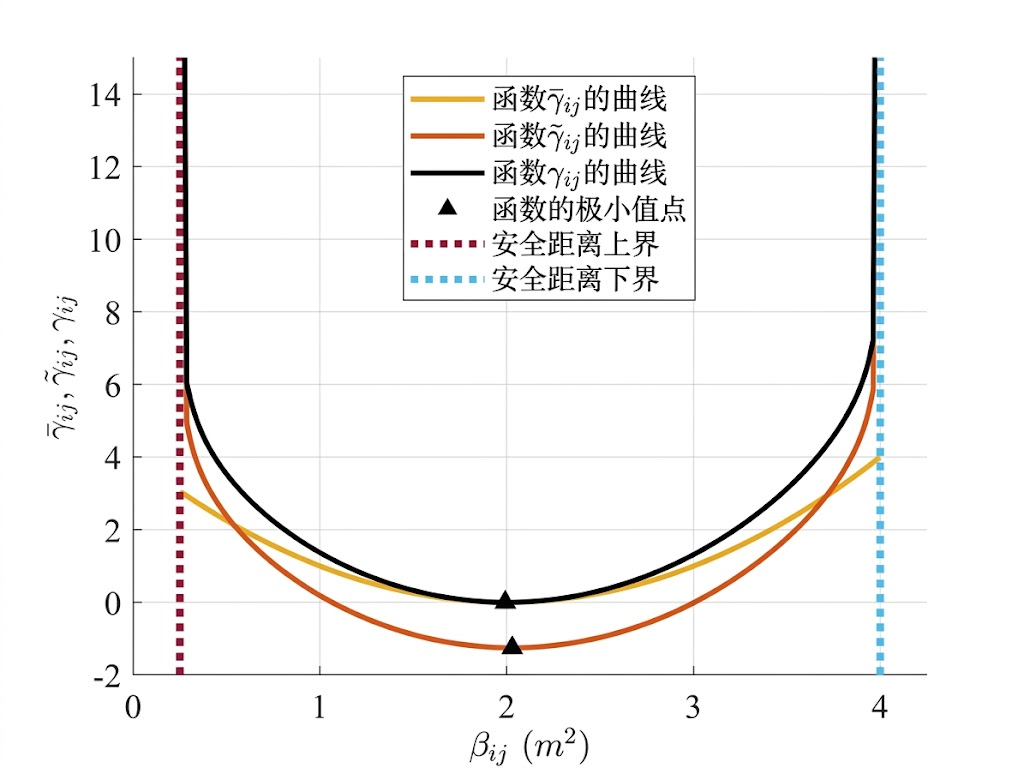
\includegraphics[width=0.75\linewidth]{images/gama函数的特性}
	\caption{$\bar{\gamma}_{ij},\tilde{\gamma}_{ij},\gamma_{ij}$函数特性对比曲线}
	\label{不同伽马函数的对比曲线}
\end{figure}



\section{稳定性证明}
考虑在上述设计的分布式观测器和控制器导引下的无人机编队，进一步分析系统的稳定性与约束保持性。为了得到整个无人机编队的闭环系统，定义无人机编队的全局势函数$\nu : \mathbb{R}^{Nn} \to \bar{\mathbb{R}}_+$为：
\begin{equation}
	\nu(\mathbf{p}) = \sum_{(i,j) \in \varepsilon} \gamma_{ij}, 
	\quad
	\mathbf{p} = [\cdots; \mathbf{p}_i; \cdots].
\end{equation}

根据分布式控制律(\ref{分布式控制律})，可得系统动力学的紧凑表达式：
\begin{equation}
	\dot{\mathbf{p}} = \mathbf{v}^* = 
	-\nabla \nu (\hat{\mathbf{p}}) - k_c(\hat{\mathbf{p}}-\mathbf{p}^*),
	\label{系统动力学紧凑表达式}
\end{equation}
式中$\mathbf{v}^*=[\cdots;\mathbf{v}_i^*;\cdots]$，$\hat{\mathbf{p}}=[\cdots;\hat{\mathbf{p}}_i;\cdots]$。接着定义矩阵$\Gamma = [\tau_{ij}] \in \mathbb{R}^{N \times N}$其中：
\begin{equation}
	\tau_{ij} =
	\begin{cases}
		-\gamma_{ij}' & \text{若}j \in \mathcal{N}_i, \\
		\sum_{s \in \mathcal{N}_i} \gamma_{is}' & \text{若}j = i, \\
		0 & \text{否则}.
	\end{cases}
\end{equation}
然后可以得到编队控制律的紧凑形式：
\begin{equation}
	\mathbf{v}^*=-\bar{\Gamma} \hat{\mathbf{p}} -k_c(\hat{\mathbf{p}}-\mathbf{p}^*),
\end{equation}
其中$\bar{\Gamma} = \Gamma \otimes I_n$。接下来对系统的输出方程(\ref{编队系统输出方程})在位置$\mathbf{p}^*$处进行线性化。省略二阶无穷小项$o (\|\mathbf{p}-\mathbf{p}^*\|^2)$，系统的输出方程可以写为：
\begin{equation}
	\mathbf{z}-\mathbf{z}^* \approx 
	\mathcal{O}_{\mathbf{p}^*}(\mathbf{p}-\mathbf{p}^*),
	\label{系统输出方程线性化}
\end{equation}
式中${\mathbf{z}}^*=[\bar{\mathbf{z}}^*;\tilde{\mathbf{z}}^*]$，其中$\bar{\mathbf{z}}^*=\frac{1}{2}[\cdots;h_{im}\|\mathbf{p}_i^*-\mathbf{p}_j^*\|^2;\cdots]$，以及$\tilde{\mathbf{z}}^*=[\cdots;\tilde{C}_i \mathbf{p}_i^*;\cdots]$。根据分布式观测器(\ref{分布式观测器})，多无人机系统的紧凑观测器形式可以写为：
\begin{equation}
	\dot{\hat{\mathbf{p}}} = 
	\mathbf{v}^* + k_o \mathcal{O}_{\mathbf{p}^*}^\top 
	[(\mathbf{z}-\mathbf{z}^*) -
	\mathcal{O}_{\mathbf{p}^*}(\hat{\mathbf{p}}-\mathbf{p}^*)].
	\label{紧凑观测器形式}
\end{equation}
接下来给出一些不等式来支撑方法的推导。首先考虑杨不等式：
\begin{equation}
	x_1^\top x_2 \le \frac{x_1^\top x_1}{2\mu} + \frac{\mu x_2^\top x_2}{2}.
	\label{杨不等式}
\end{equation}
对于$x_1 \in \mathbb{R}^n$，$x_2 \in \mathbb{R}^n$，以及任意正常数$\mu$，上述不等式成立。另外，不等式：
\begin{equation}
	x^\top \mathbf{P}_1 x \le
	\lambda_\text{max}(\mathbf{P}_2^{-1} \mathbf{P}_1)x^\top \mathbf{P}_2 x \le
	\frac{\|\mathbf{P}_1\|_2}
	{\|\mathbf{P}_2\|_2}x^\top \mathbf{P}_2 x.
	\label{不等式1}
\end{equation}
对任意的对称矩阵$\mathbf{P}_1 \in \mathbb{R}^{n \times n}$和任意的正定矩阵$\mathbf{P}_2 \in \mathbb{R}^{n \times n}$成立。

接下来通过下述定理阐明本节所设计控制方法的稳定性。

\textbf{定理4.1.} 根据给定的期望无穷小刚性编队框架$\mathcal{F}^*$，考虑无人机一阶动力学(\ref{一阶动力学})，在分布式观测器(\ref{分布式观测器})和控制器(\ref{分布式控制律})的驱动下，如果反馈增益矩阵满足条件(\ref{控制反馈增益条件})和(\ref{观测反馈增益条件})，那么系统可在初值邻域条件(\ref{初值邻域条件})下局部收敛至期望编队$\mathcal{F}^*$。

\textit{证明：}

首先定义编队的位置控制误差为 $\bar{\mathbf{p}} = \mathbf{p} - \mathbf{p}^*$，位置估计误差为 $\tilde{\mathbf{p}} =\mathbf{p}- \hat{\mathbf{p}}$。构建如下包含编队势能和系统动能的候选李雅普诺夫函数：
\begin{equation}
	V = \sum_{(i,j) \in \varepsilon} \gamma_{ij} + 
	\frac{k_c}{2} \bar{\mathbf{p}}^\top \bar{\mathbf{p}} + \frac{k_o}{2} \tilde{\mathbf{p}}^\top \tilde{\mathbf{p}}
\end{equation}
定义$V_1=\sum_{(i,j) \in \varepsilon}\gamma_{ij}$，$V_2=\frac{k_c}{2} \bar{\mathbf{p}}^\top \bar{\mathbf{p}}$，以及$V_3=\frac{k_o}{2} \tilde{\mathbf{p}}^\top \tilde{\mathbf{p}}$。接着定义$\mathcal{W}=\text{diag}\{\dots,\gamma_{ij}',\dots\}$和$\mathbf{e}=[\cdots;\mathbf{e}_{ij};\cdots]$，其中$\mathbf{e}_{ij}=\mathbf{p}_i-\mathbf{p}_j$，可以得到$\Gamma=\mathcal{H}\mathcal{W}\mathcal{H}^\top$和$\mathbf{e}=(\mathcal{H}^\top \otimes I_n)\mathbf{p}$，并推导出：
\begin{align}
	\dot{V_1} &= 
	\left[(\mathcal{W} \otimes I_n)\mathbf{e}\right]^\top
	(\mathcal{H}^\top \otimes I_n)\dot{\mathbf{p}} \nonumber \\
	&=
	-\mathbf{p}^\top(\mathcal{H}\mathcal{W}\mathcal{H}^\top \otimes I_n)
	\left[\bar{\Gamma}\hat{\mathbf{p}}+k_c(\hat{\mathbf{p}}-\mathbf{p}^*)\right] \nonumber \\
	&=
	-(\hat{\mathbf{p}}+\tilde{\mathbf{p}})^\top \bar{\Gamma}^2 \tilde{\hat{p}} - k_c(\hat{\mathbf{p}}+\tilde{\mathbf{p}})^\top \bar{\Gamma} (\hat{\mathbf{p}}-\mathbf{p}^*),
	\label{V1导数}
\end{align}
\begin{align}
	\dot{V_2} &=
	-k_c(\mathbf{p}-\mathbf{p}^*)^\top
	\left[\bar{\Gamma}\hat{\mathbf{p}}+k_c(\hat{\mathbf{p}}-\mathbf{p}^*)\right] \nonumber \\
	&= 
	-k_c(\hat{\mathbf{p}}-\mathbf{p}^*)^\top \bar{\Gamma}\hat{\mathbf{p}} -
	k_c^2(\hat{\mathbf{p}}-\mathbf{p}^*)^\top (\hat{\mathbf{p}}-\mathbf{p}^*) - 
	k_c \tilde{\mathbf{p}}^\top \bar{\Gamma} \hat{\mathbf{p}} - 
	k_c^2 \tilde{\mathbf{p}}^\top (\hat{\mathbf{p}}-\mathbf{p}^*),
	\label{V2导数}
\end{align}
以及
\begin{equation}
	\dot{V_3} = 
	k_o \tilde{\mathbf{p}}^\top \dot{\tilde{\mathbf{p}}} = 
	-k_o^2 \tilde{\mathbf{p}}^\top \mathcal{O}_{\mathbf{p}^*}^\top
	\mathcal{O}_{\mathbf{p}^*} \tilde{\mathbf{p}}.
	\label{V3导数}
\end{equation}
随后结合公式(\ref{V1导数})，(\ref{V2导数})以及(\ref{V3导数})，可以得到函数$V$沿无人机编队系统轨迹随时间演变的导数：
\begin{align}
	\dot{V} &= -\hat{\mathbf{p}}^\top \left( {\Gamma}^2 \otimes I_n \right) \hat{\mathbf{p}} - 2k_c \hat{\mathbf{p}}^\top \left( \hat{\mathbf{p}} - \mathbf{p}^* \right) - k_c^2 \left( \hat{\mathbf{p}} - \mathbf{p}^* \right)^\top \left( \hat{\mathbf{p}} - \mathbf{p}^* \right) - \tilde{\mathbf{p}}^\top \left( \bar{\Gamma}^2 + k_c \bar{\Gamma} \right) \hat{\mathbf{p}} \notag \\
	&\quad - \tilde{\mathbf{p}}^\top \left[ k_c \bar{\Gamma} + k_c^2 I_{Nn} \right] \left( \hat{\mathbf{p}} - \mathbf{p}^* \right) - k_o^2 \tilde{\mathbf{p}}^\top \mathcal{O}_{\mathbf{p}^*}^\top \mathcal{O}_{\mathbf{p}^*} \tilde{\mathbf{p}} \notag \\
	&= - \left[ \bar{\Gamma} \hat{\mathbf{p}} + k_c \left( \hat{\mathbf{p}} - \mathbf{p}^* \right) \right]^\top \left[ \bar{\Gamma} \hat{\mathbf{p}} + k_c \left( \hat{\mathbf{p}} - \mathbf{p}^* \right) \right] - \tilde{\mathbf{p}}^\top \left[ \bar{\Gamma} + k_c I_{Nn} \right] \left[ \bar{\Gamma} \hat{\mathbf{p}} + k_c \left( \hat{\mathbf{p}} - \mathbf{p}^* \right) \right] \notag \\
	&\quad - k_o^2 \tilde{\mathbf{p}}^\top \mathcal{O}_{\mathbf{p}^*}^\top \mathcal{O}_{\mathbf{p}^*} \tilde{\mathbf{p}}.
	\end{align}
应用杨不等式(\ref{杨不等式})，可以推导出：
\begin{equation}
	\dot{V} \le -\tilde{\mathbf{p}}^\top 
	\left[
		k_o^2 \mathcal{O}_{\mathbf{p}^*}^\top \mathcal{O}_{\mathbf{p}^*}
		-\frac{(\bar{\Gamma}+k_c I_{Nn})^2}
		{2 \mu_1}	
	\right]
	\tilde{\mathbf{p}}
	-k_{\mu_1} {\mathbf{v}^*}^\top {\mathbf{v}^*},
	\label{不等式2}
\end{equation}
式中$k_{\mu_1}=\frac{2-\mu_1}{2},0<\mu_1<2$。进一步计算函数$\gamma_{ij}''$：
\begin{equation}
	\gamma_{ij}'' = k_\gamma
	\left[
		2+\frac{(\rho_{e_2}^2-\beta_{ij})^2+(\beta_{ij}-\rho_{e_1}^2)^2}
		{[(\rho_{e_2}^2-\beta_{ij})(\beta_{ij}-\rho_{e_1}^2)]^2}
	\right]
	>0.
\end{equation}
由此可知，函数$\gamma_{ij}'$是单调递增的。接下来考虑编队期望位置的邻域：
\begin{equation}
	\mathcal{U}_\mathbf{p} = 
	\{
		\mathbf{p} \in \mathbb{R}^{Nn}:\|\mathbf{p}_i-\mathbf{p}_i^*\|
		\le \rho_\mathbf{p}
	\},
\end{equation}
其中$\rho_\mathbf{p}$为正常数并且满足：
\begin{equation}
	\rho_{e_1}^2 < \beta_{ij}^* \pm 4\rho_\mathbf{p}
	(\rho_\mathbf{p}+|\mathbf{e}^*|_\infty) <\rho_{e_2}^2.
	\label{初值邻域条件}
\end{equation}
其中$\mathbf{e}^*=[\dots;\mathbf{e}^*_{ij};\dots]$，以及$\mathbf{e}_{ij}^*=\mathbf{p}_i^*-\mathbf{p}_j^*$。进一步可推导得：
\begin{equation}
	|\beta_{ij}-\beta_{ij}^*| = 
	|(\mathbf{e}_{ij}+\mathbf{e}^*_{ij})^\top(\mathbf{e}_{ij}-\mathbf{e}^*_{ij})| \le 
	4\rho_\mathbf{p}
	(\rho_\mathbf{p}+|\mathbf{e}^*|_\infty),
\end{equation}
以及
\begin{equation}
	\|\gamma_{ij}'\| \le
	2\rho_\gamma(\rho_\mathbf{p}+|\mathbf{e}^*|_\infty)
	\|\mathbf{e}_{ij}-\mathbf{e}^*_{ij}\| \le
	4\rho_\mathbf{p} \rho_\gamma
	(\rho_\mathbf{p}+|\mathbf{e}^*|_\infty),
\end{equation}
其中$\rho_\gamma=\text{max}\{|\gamma_{ij}''(\beta_{ij}^*\pm4\rho_\mathbf{p}(\rho_\mathbf{p}+|\mathbf{e}^*|_\infty))|\}$。然后可以得到：
\begin{equation}
	\|\bar{\Gamma}\|_2 \le
	\|\mathcal{H}\mathcal{W}\mathcal{H}^\top\|_2 \le
	4 \rho_\gamma \rho_\mathbf{p}
	(\rho_\mathbf{p}+|\mathbf{e}^*|_\infty)\|\mathcal{H}\|^2_2.
\end{equation}
该式意味着$\|\bar{\Gamma}\|_2$具有上界：
\begin{equation}
	\rho_\Gamma = 
	4\rho_\gamma \rho_\mathbf{p} 
	(\rho_\mathbf{p}+|\mathbf{e}^*|_\infty)\|\mathcal{H}\|^2_2
\end{equation}
注意到矩阵$\mathcal{O}_{\mathbf{p}^*}^\top \mathcal{O}_{\mathbf{p}^*}$的正定性和矩阵$\Gamma$的对称性，参考不等式(\ref{不等式1})，可以得到：
\begin{equation}
	\tilde{\mathbf{p}}^\top
	\left[
		\frac{(\bar{\Gamma}+k_c I_{Nn})^2}
		{2 \mu_1}
	\right]
	\tilde{\mathbf{p}}
	\le
	\frac{(\rho_\Gamma+k_c)^2}
	{2\mu_1 \|\mathcal{O}_{\mathbf{p}^*}\|^2_2}
	\tilde{\mathbf{p}}^\top
	(\mathcal{O}_{\mathbf{p}^*}^\top \mathcal{O}_{\mathbf{p}^*})
	\tilde{\mathbf{p}}.
\end{equation}
此时，不等式(\ref{不等式2})可缩放为：
\begin{equation}
	\dot{V} \le
	-\left[
		k_o^2 -
		\frac{(\rho_\Gamma+k_c)^2}
		{2\mu_1 \|\mathcal{O}_{\mathbf{p}^*}\|^2_2}
	\right]
	\tilde{\mathbf{p}}^\top
	(\mathcal{O}_{\mathbf{p}^*}^\top \mathcal{O}_{\mathbf{p}^*})
	\tilde{\mathbf{p}}
	-k_{\mu_1}
	{\mathbf{v}^*}^\top {\mathbf{v}^*}.
\end{equation}
再次结合杨不等式(\ref{杨不等式})进一步得：
\begin{align}
	\dot{V}
	&\leq -\left[ k_o^2 - \frac{(\rho_\Gamma + k_c)^2}{2\mu_1 \|\mathcal{O}_{\mathbf{p}^*}\|_2^2} \right]
	\tilde{\mathbf{p}}^\top (\mathcal{O}_{\mathbf{p}^*}^\top \mathcal{O}_{\mathbf{p}^*}) \tilde{\mathbf{p}}
	- k_{\mu_1} k_{\mu_2} k_c^2 (\hat{\mathbf{p}} - \mathbf{p}^*)^\top (\hat{\mathbf{p}} - \mathbf{p}^*) \nonumber \\
	&\quad + 2k_{\mu_1} k_{\mu_2} \mu_2 \|\bar{\Gamma}^2\|_2^2 \left( \|\tilde{\mathbf{p}}\|^2 + \|\mathbf{p}\|^2 \right) \nonumber \\
	&\leq -\left[ k_o^2 \|\mathcal{O}_{\mathbf{p}^*}\|_2^2 - \frac{(\rho_\Gamma + k_c)^2}{2\mu_1}
	- 2k_{\mu_1} k_{\mu_2} \mu_2 (\rho_\Gamma^2 + \rho_c^2) \right] \|\tilde{\mathbf{p}}\|^2 \nonumber \\
	&\quad - k_{\mu_1} k_{\mu_2} \left( k_c^2 - 2\mu_2 \rho_c^2 \right) \|\hat{\mathbf{p}} - \mathbf{p}^*\|^2,
	\label{不等式3}
\end{align}
式中$k_{\mu_2}=\frac{\mu_2-1}{\mu_2},\mu_2>1$以及$\rho_c=2\rho_\gamma\rho_{e_2}(\rho_\mathbf{p}+|\mathbf{e}^*|_\infty)\|\mathcal{H}\|^2_2$。如果反馈增益满足条件：
\begin{equation}
	k_c>\sqrt{2\mu_2}\rho_c,
	\label{控制反馈增益条件}
\end{equation}
以及
\begin{equation}
	k_o > \sqrt{ \frac{(\rho_\Gamma + k_c)^2}{2\mu_1 \|\mathcal{O}_{p^*}\|_2^2} + \frac{2k_{\mu_1}(\mu_2 - 1)(\rho_\Gamma^2 + \rho_c^2)}{\|\mathcal{O}_{p^*}\|_2^2} }
	\label{观测反馈增益条件}
\end{equation}
在不等式(\ref{不等式3})基础上可推得$\dot{V}\le0$成立。进一步，如果$\|\hat{\mathbf{p}}-\mathbf{p}^*\|\neq0$或者$\|\mathbf{p}-\hat{\mathbf{p}}\|\neq0$，可以得到:
\begin{equation}
	\dot{V}<0
\end{equation}
由此说明位置误差$\bar{\mathbf{p}}$和估计误差$\tilde{\mathbf{p}}$的局部渐进收敛性。
